% =====================================================================
%  Galton-board slide: a single run vs. the program as a whole.
%
%  Embeds two videos generated by figs/galton_video.py:
%    figs/single.mp4  (95 frames, frame_0 .. frame_94)
%    figs/swarm.mp4   (287 frames, frame_0 .. frame_286)
%
%  Each video is embedded two ways; keep whichever plays in your viewer:
%    (a) multimedia \movie -- a "Screen annotation" pdfpc plays natively.
%        CLICK the poster (frame_0) to play; pdfpc has no autoplay and
%        resets the movie when you leave the slide. Needs GStreamer with
%        an H.264 decoder installed (gstreamer1.0-libav + -plugins-bad).
%    (b) \animategraphics PNG-sequence fallback -- Adobe Reader only.
%  The \animategraphics lines are commented out by default.
%
%  Requires \usepackage{multimedia} and \usepackage{animate} in the
%  preamble (animate is already loaded in main.tex).
% =====================================================================
\begin{frame}{A program is a distribution over runs}

  % ---- Title bar: the type of flip -----------------------------------
  \begin{center}
    $\mathrm{flip} : (m : \mathbb{R}) \to \mathrm{Distrib}\ \{m, m+1\}$
  \end{center}
  \vspace{0.4em}

  \begin{columns}[T]

    % ================= LEFT: single ball =============================
    \begin{column}{0.32\textwidth}
      \centering
      {\small \wprob{an individual ``run'' of the program}}\\[0.3em]

      \movie[loop, showcontrols]%
        {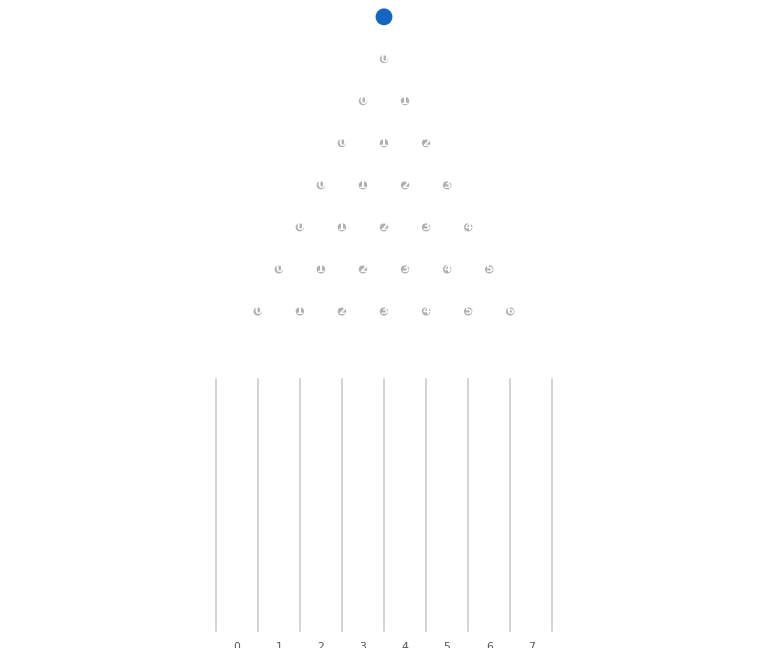
\includegraphics[width=0.92\linewidth]{figs/frame_0.png}}%
        {figs/single.mp4}
      % --- Adobe-Reader-only fallback (comment the \movie above to use) ---
      % \animategraphics[autoplay,loop,width=0.92\linewidth]{25}{figs/single/frame_}{0}{94}

      \vspace{0.3em}

      {\small \wprob{Honing in on a single marble}}
    \end{column}

    % ================= MIDDLE: pseudocode ============================
    \begin{column}{0.34\textwidth}
      \centering
      \vspace{1.6em}
      \[
        \begin{aligned}
          X_0 &\leftarrow \mathrm{flip}\ 0\\
          X_1 &\leftarrow \mathrm{flip}\ X_0\\
          X_2 &\leftarrow \mathrm{flip}\ X_1\\
          \mathrm{ret}&\ X_2
        \end{aligned}
      \]
      \vspace{0.2em}

      {\Large $\mathrel{|\,|\,|}$}
      \vspace{0.4em}

      \[
        \mathrm{for}\ (3,\ \mathrm{flip}\ 0,\ \lambda X.\ \mathrm{flip}\ X)
      \]
    \end{column}

    % ================= RIGHT: swarm ==================================
    \begin{column}{0.32\textwidth}
      \centering
      {\small \wprob{The program as a whole}}\\[0.3em]

      \movie[loop, showcontrols]%
        {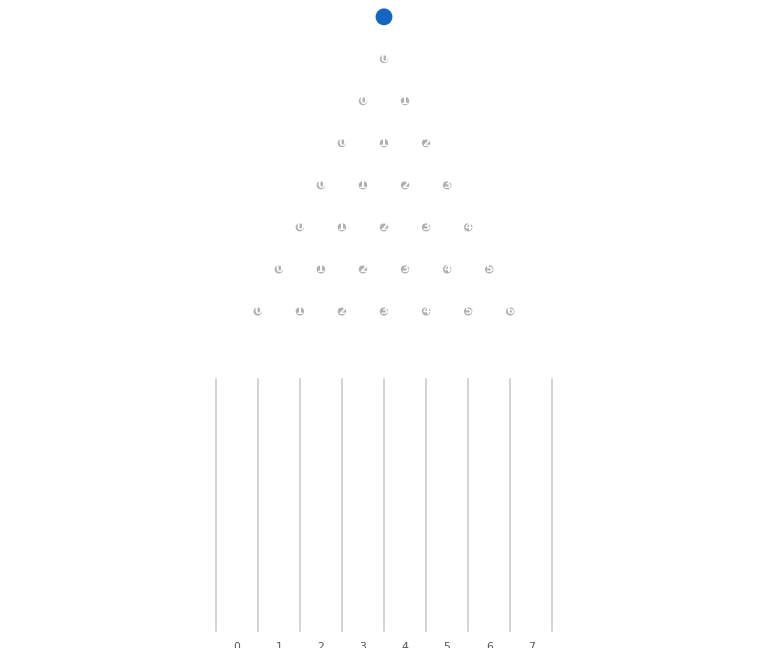
\includegraphics[width=0.92\linewidth]{figs/frame_0.png}}%
        {figs/swarm.mp4}
      % --- Adobe-Reader-only fallback (comment the \movie above to use) ---
      % \animategraphics[autoplay,loop,width=0.92\linewidth]{25}{figs/swarm/frame_}{0}{286}

      \vspace{0.3em}

      {\small \wprob{All the marbles at once}}
    \end{column}

  \end{columns}
\end{frame}
